\newpage


\section{Moderne Cyberbedrohungen}\label{sec:moderne-cyberbedrohungen}
%\todo[inline]{Eventuell Einleitungstext schreiben}

\subsection{Trends in der Cyberkriminalität}\label{subsec:trends-und-entwicklungen-in-der-cyberkriminalitat}
In den letzten Jahren hat die Anzahl der Cyberkriminalitätsfälle in Deutschland stark zugenommen.
So wurden zwar für das Jahr $2022$ ein Rückgang von 6.5\% gegenüber dem Vorjahr an erfassten Fällen aufgezeichnet, jedoch bildet sich in dem Zeitraum von $2012$ bis $2022$ ein Gesamtwachstum von 112\% an erfassten Cyberkriminalitätsfällen\autocite[\vglf][]{bka-cyberkriminalitaet}.

Analog zu der Anzahl der aufgezeichneten Fälle steigen auch die Kosten, die Cyberkriminalität verursacht, sowie die Ausgaben die für IT-Sicherheit in Deutschland vorgenommen werden stetig.
$2018$ haben Cyberkriminalitätsvorfälle deutschen Unternehmen durchschnittlich $13,12$ Millionen US-Dollar\footnote{Heutiger Wert ungefähr $10,23$ Millionen Euro} gekostet, was gegenüber dem Vorjahr ein Zuwachs von fast 18\% darstellt\autocite[\vglf][]{accenture-cyberkrime-kosten}.
$2021$ wurden so ungefähr $6,9$ Milliarden Euro für IT-Sicherheitsmaßnahmen ausgegeben, was einem Zuwachs von fast 22\% gegenüber dem Vorjahr entspricht\autocite[\vglf][]{bitkom-itsicherheit}, davon wurden geschätzt $1,7$ Milliarden Euro für Softwarelösungen ausgegeben\autocite[\vglf][]{bitkom-itsicherheit-segment}.

Wie die Kosten und Ausgaben für Cyberkriminalität steigen auch die möglichen Methoden der Angreifer.
\autoref{fig:cybercrime-chart-absolute} zeigt nach den Statista Market Insights\autocite[\vglf][]{statista-cybersecurity-cybercrime}, dass die Anzahl der Fälle von Cyberkriminalität fast stetig zunimmt.

\begin{figure}[htpb]
    \centering
    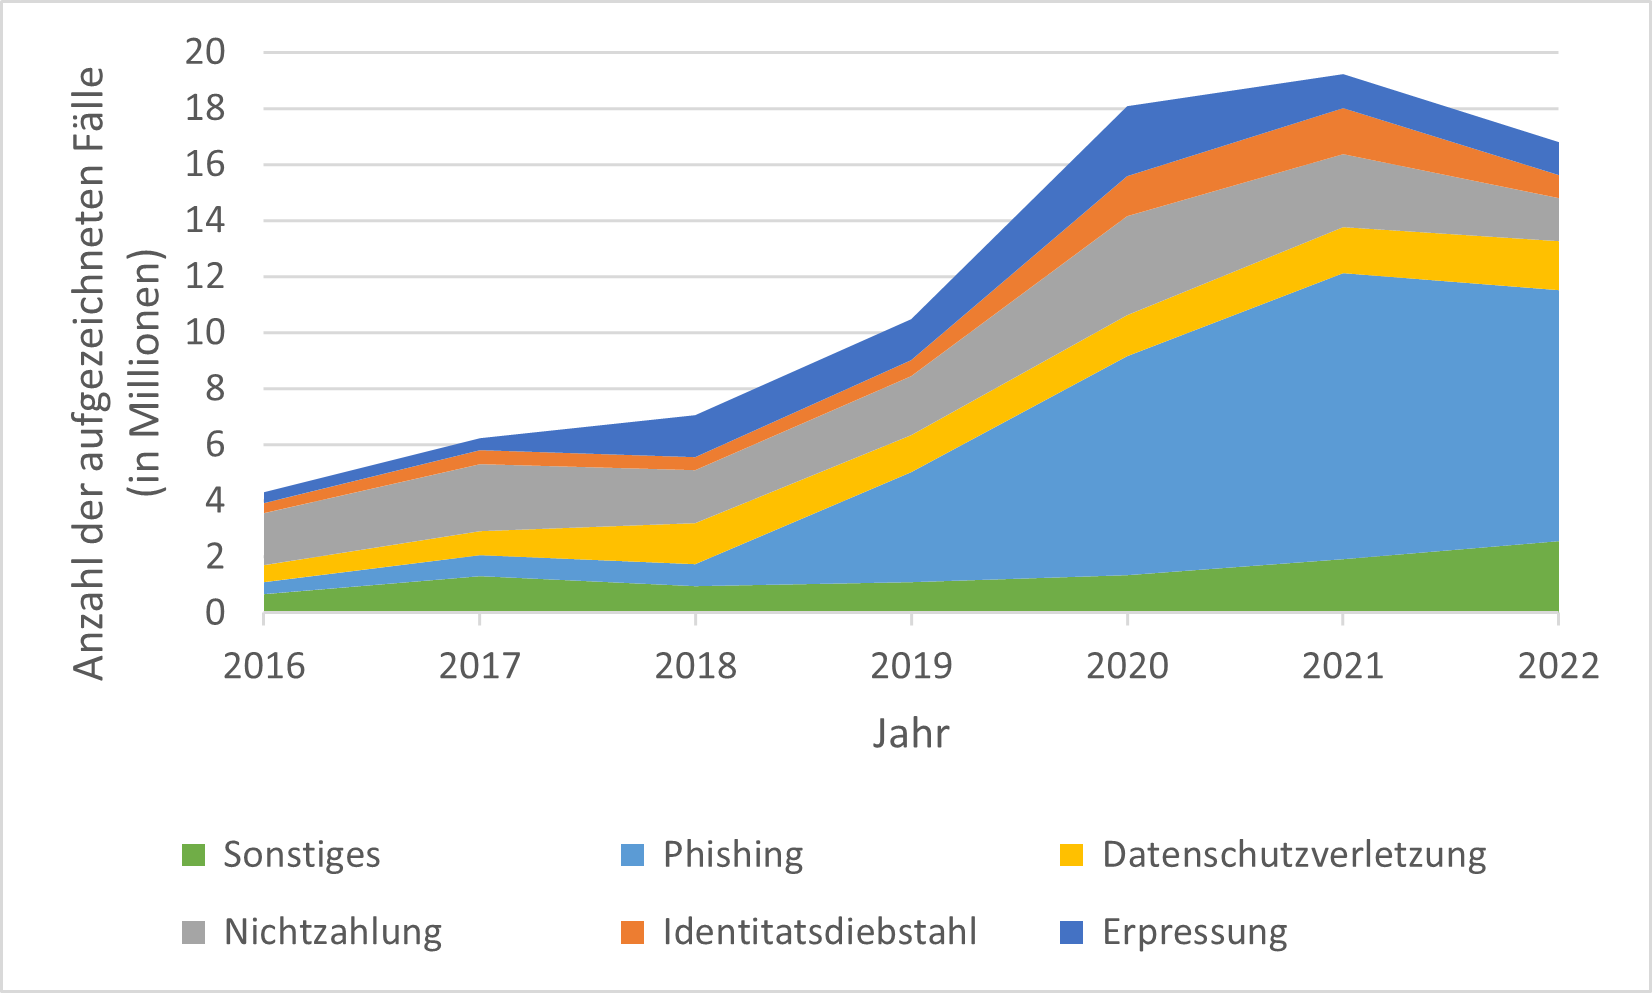
\includegraphics[width = 0.75\linewidth, trim = {0.55cm 0.3cm 0.4cm 0.25cm}, clip]{src/abbildungen/Aufgezeichnete_Cyberkriminalitaet}
    \captionsetup{width=\linewidth, format=hang}
    \caption[Erfasste Fälle von Cyberkriminalität nach Typ]{Erfasste Fälle von Cyberkriminalität nach Typ.\newline Stand September 2023}
    \label{fig:cybercrime-chart-absolute}
\end{figure}

Einzig im Jahr $2022$ wurde ein Rückgang der erfassten Fälle aufgezeichnet.
Besonders der Anteil, der Phishingangriffe hat im Vergleich zu $2018$ stark zugenommen, wohingegen die Nichtzahlung von Leistungen stark abgenommen hat, wie in \autoref{fig:cybercrime-chart-relative} aus den Statista Market Insights\autocite[\vglf][]{statista-cybersecurity-cybercrime} dargestellt wird.

\begin{figure}[htpb]
    \centering
    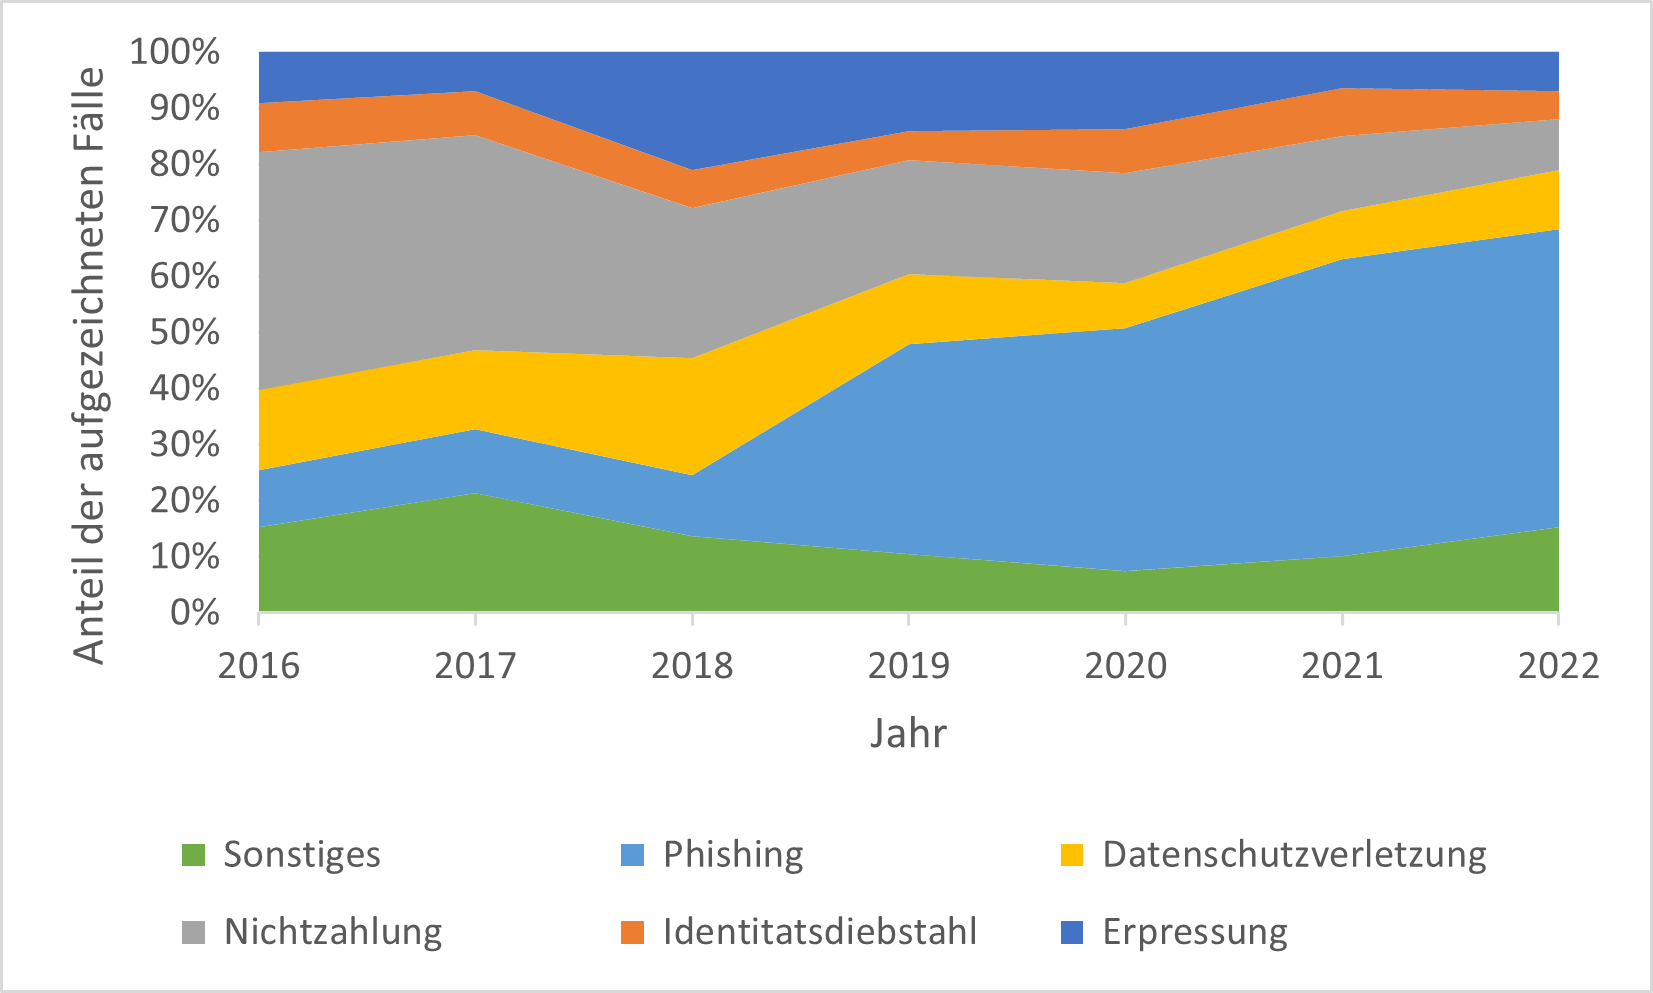
\includegraphics[width = 0.75\linewidth, trim = {0.55cm 0.3cm 0.4cm 0.25cm}, clip]{src/abbildungen/Anteile_Cyberkriminalitaet}
    \captionsetup{width=\linewidth, format=hang}
    \caption[Anteil einzelner Cyberkriminalitätstypen]{Anteil einzelner Cyberkriminalitätstypen.\newline Stand September 2023}
    \label{fig:cybercrime-chart-relative}
\end{figure}

\subsection[Arten von Cyberbedrohungen]{Arten von Cyberbedrohungen - Malware, Phishing, DDoS}\label{subsec:arten-von-cyberbedrohungen---malware-phishing-ddos}

Die drei häufigsten Methoden von Cyberattacken sind Malware, Phishing und \ac{ddos} Angriffe.

\begin{definition}
    \label{def:phishing}
    Phishing bezeichnet den Versuch, an vertrauliche Informationen wie Anmeldedaten oder Kreditkarteninformationen zu gelangen, indem ein System innerhalb eines Kommunikationsvorgangs als vertrauenswürdig ausgibt.\autocite[\vglf][\pagef 27]{study-on-phishing-attacks:2018}
\end{definition}

\begin{definition}
    \label{def:malware}
    Malware bezeichnet eine Software, welche ausschließlich Systeme angreift, welche entweder keine anderen Systeme beschädigen, oder welche Malwaresysteme angreifen.\autocite[\vglf][\pagef 108f.]{definition-malware-2010}
\end{definition}

\begin{definition}
    \label{def:ddos}
    Unter \ac{ddos}-Angriffen werden Vorgänge verstanden, gezielt versuchen, ein Netzwerk oder einen Computer die Möglichkeit zu nehmen, gewohnte Dienste auszuführen.
    Bei solchen Angriffen werden die vorhandenen Daten und Systeme weder direkt noch permanent angegriffen, es wird lediglich die Verfügbarkeit dieser Ressourcen unterbunden.\autocite[\vglf][\pagef 190]{ddos-definition-2003}
\end{definition}

Diese Angriffe zielen auf verschiedene Angriffsflächen und haben verschiedene Ziele, welche das korruptieren von Daten oder Systeme oder das Hindern des Zugriffs auf Daten und Systeme beinhalten können.
Um diese Angriffe abzuwehren, gibt es verschiedene Methoden, eine davon ist eine \ac{zta}.

